\chapter{Method}
\label{chap:method}

\section{Data Collection}
\label{sec:data}
The experiment was hosted through an open-source crowdsourcing client/system server system LingoTurk \citep{lingoturk}.
The participants were recruited via Prolific \citep{prolific}, a subject pool for online experiments. The following criteria were used to filter the participants: native English speaker located in the UK, age in range 18-40, minimal approval rate of 95\%, number of previous submissions must be at least 20 studies, participants cannot have taken part in any of the related studies our group has conducted before. The estimated length of the experiment was 22 minutes, with the median completion time being 19 minutes and 30 seconds. The participants were paid 3.89 pounds which is equivalent to minimal hour wage in Germany. The participants were paid only in case of successful completion of the full experiment. The experiment was conducted in a web browser and the participants were asked to use a computer with functional webcam. The project was approved by the Ethical Review Board of the Faculty of Mathematics and Computer Science at Saarland University.


\subsection{Reference Games}
\label{sec:data:ref_games}
There were 3 conditions of the reference games used in this experiment: Simple, Complex and Unambiguous. In the \autoref{sec:rsa} we mainly talked about the Simple and Complex conditions. The Unambiguous condition serves two main purposes. First of all, it acts as a sort of filler, so that participants do not get used to the same type of problems. Second of all, it acts as a control check, that is, participants who do not reach 75\% accuracy on the Unambiguous trials are excluded from the analysis.

The trials were generated using 3 colors: red, green and blue, and 3 shapes: square, circle and triangle. The code used to generate trials can be found under the folder ``trials'' \citep{github}. For each condition every unique sent message was repeated exactly twice. Which results in 12 trials of every condition. Another restriction we included was that available messages always have 2 shapes and 2 colors. Furthermore one Simple and one Complex trial was picked to be repeated once again in the very end of the experiment. These were, so called, strategy trials where we would ask the participants to explain their reasoning behind the choice of the object, a similar approach was incorporated in the study by \cite{Mayn_2023}. All trials were randomly shuffled before the experiment, except for the strategy trials which were always at the end of the experiment. The full list of trials is shown in in \autoref{tab:trials}. 

In addition, a feedback system was incorporated in the trials. After every answer a pop up at the top of the screen would show up for 1200 ms. It would only show ``Correct'' or ``Incorrect'', based on whether the participant chose the Target or not. No other feedback was given during the experiment. The strategy trials did not include this feature at all. 

\begin{figure}
    \centering
    \fbox{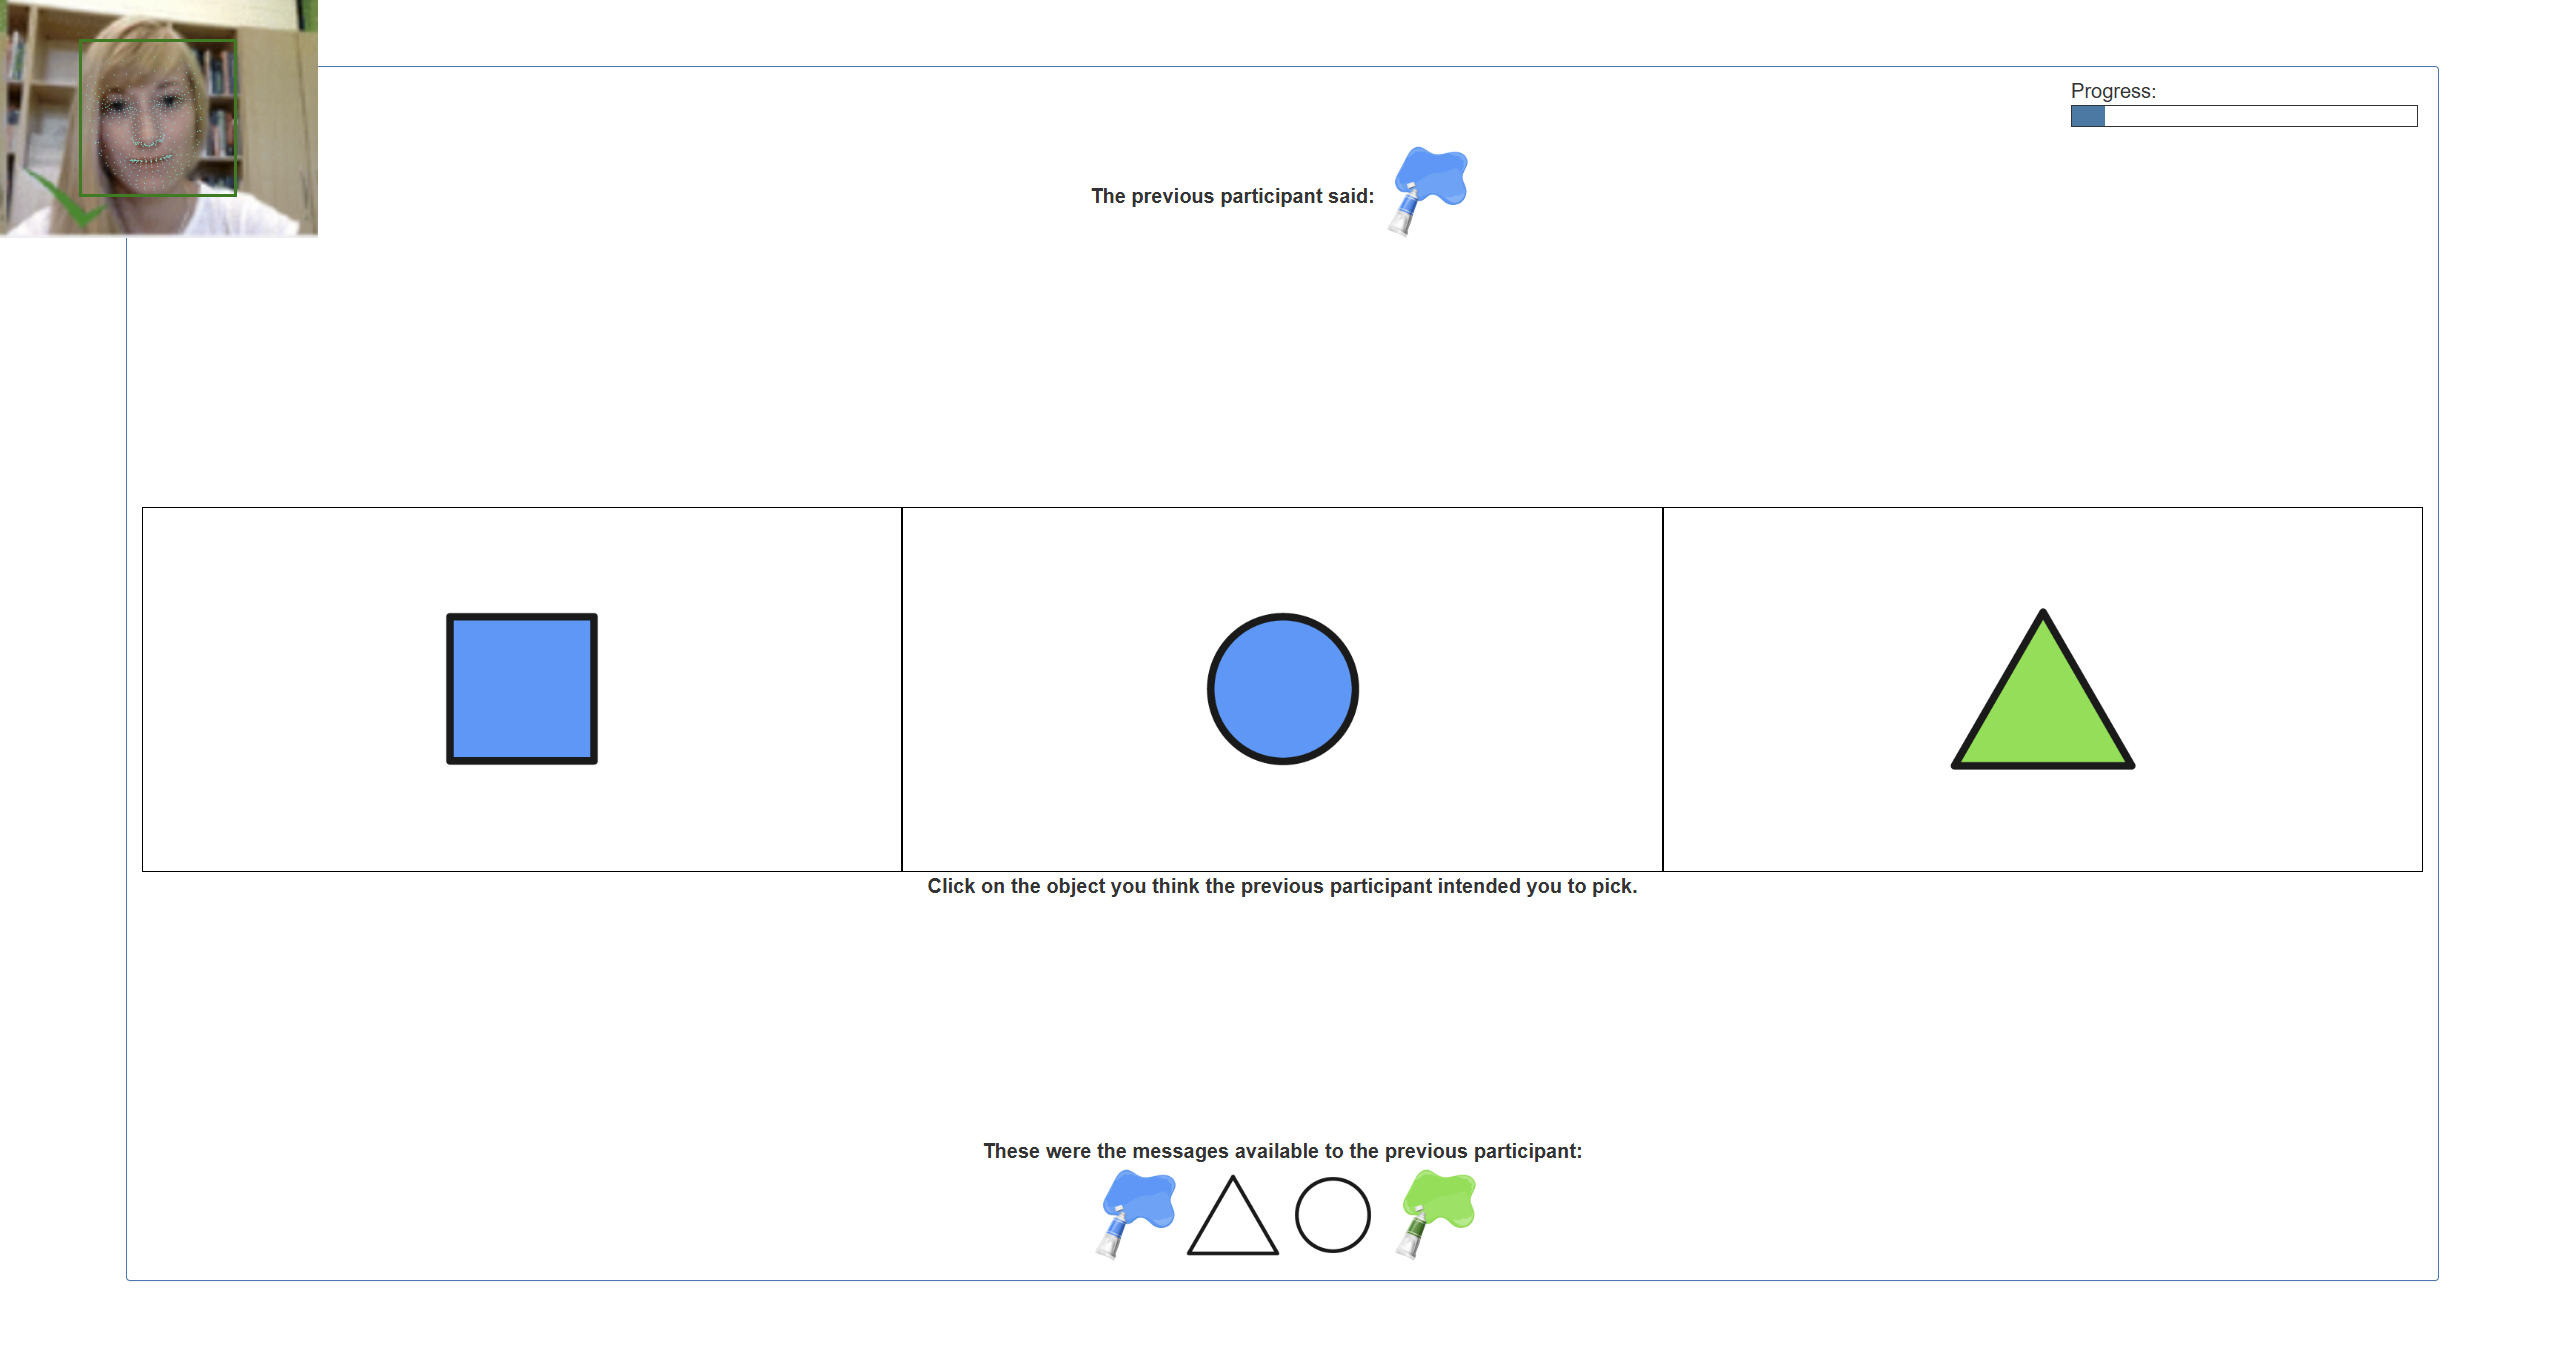
\includegraphics[width=0.8\textwidth]{images/example_trial_webcam.png}}
    \caption{Example trial}
    \label{fig:example_trial_webcam}
\end{figure}

Before the main part of the experiment with 36 + 2 trials, the participants were asked to do a speaker's job in reference games with 3 Unambiguous trials and 1 completely ambiguous one. The participants were asked to describe the object in the ambiguous trial in a way that the listener would be able to pick the correct object. Later they were told that a previous participant had already done the speaker's job and they were to do the listener's job, which was the main part of the experiment with 36 + 2 trials. An example trial can be seen in \autoref{fig:example_trial_webcam}. Depending on the zoom and the resolution of the page, the sizes and absolute positions of the images would vary a lot. Hence, the absolute positions in pixels as well as sizes of the images were saved during the experiment. 

\subsection{Eye Tracking}
\label{sec:data:eyetr}
The eye tracking was done via library WebGazer \citep{webgazer}. The library was used to track participants' gaze on the screen. The library is implemented as a linear regression model to predict x and y coordinates based on encoded gaze and facial features. There was a calibration in the beginning of the experiment after the practice trials where participants did the speaker's job, this allowed to put the calibration as close to the main experiment as possible. The calibration was adapted from the one used in the demo of WebGazer \citep{webgazer}. During the calibration participants are asked to click on the points, every click is used to adjust the model parameters to the particular setup. The calibration works based on the assumption that people would look where they click. We included 11 points instead of 9 as in the demo, the additional points were put on the objects' places. Each point had to be clicked 5 times. The setup can be seen in \autoref{fig:calibration_webcam}.In addition, the calibration accuracy assessment in the end was done not with 1 point but 3: middle, left and right. Where left and right again correspond to the positions of the main objects on the screen. Furthermore, an in-between trial calibration was incorporated to ensure that the calibration was still accurate. This drastically improves the performance of the model as during the experiment participants would make small or not adjustments which would make the initial calibration not as accurate as they progress through the experiment. However, including the in-between calibration solves this problem as right before the trial, participants click and by assumption look at the places where the areas of interest are located making the model adjust to the current setup. The model only saves last 50 clicks and replaces the oldest ones one by one after more than 50 were done. During the in-between calibration the number of points were reduced to 5, each point corresponding to one of the areas of interest. No accuracy assessment was performed during the in-between trial calibration. The setup can be seen in \autoref{fig:inbetween_calibration_webcam}. In order to make the first fixation after the in-between calibration more predictable, the top point, that corresponds to the sent message, was not available until all the other points were clicked on. This way participants would enter the trial looking at the sent message which is we expected to be the first point of interest. The sent message gives crucial information about the trial without which it is impossible to solve the task.

\begin{figure}
    \centering
    \fbox{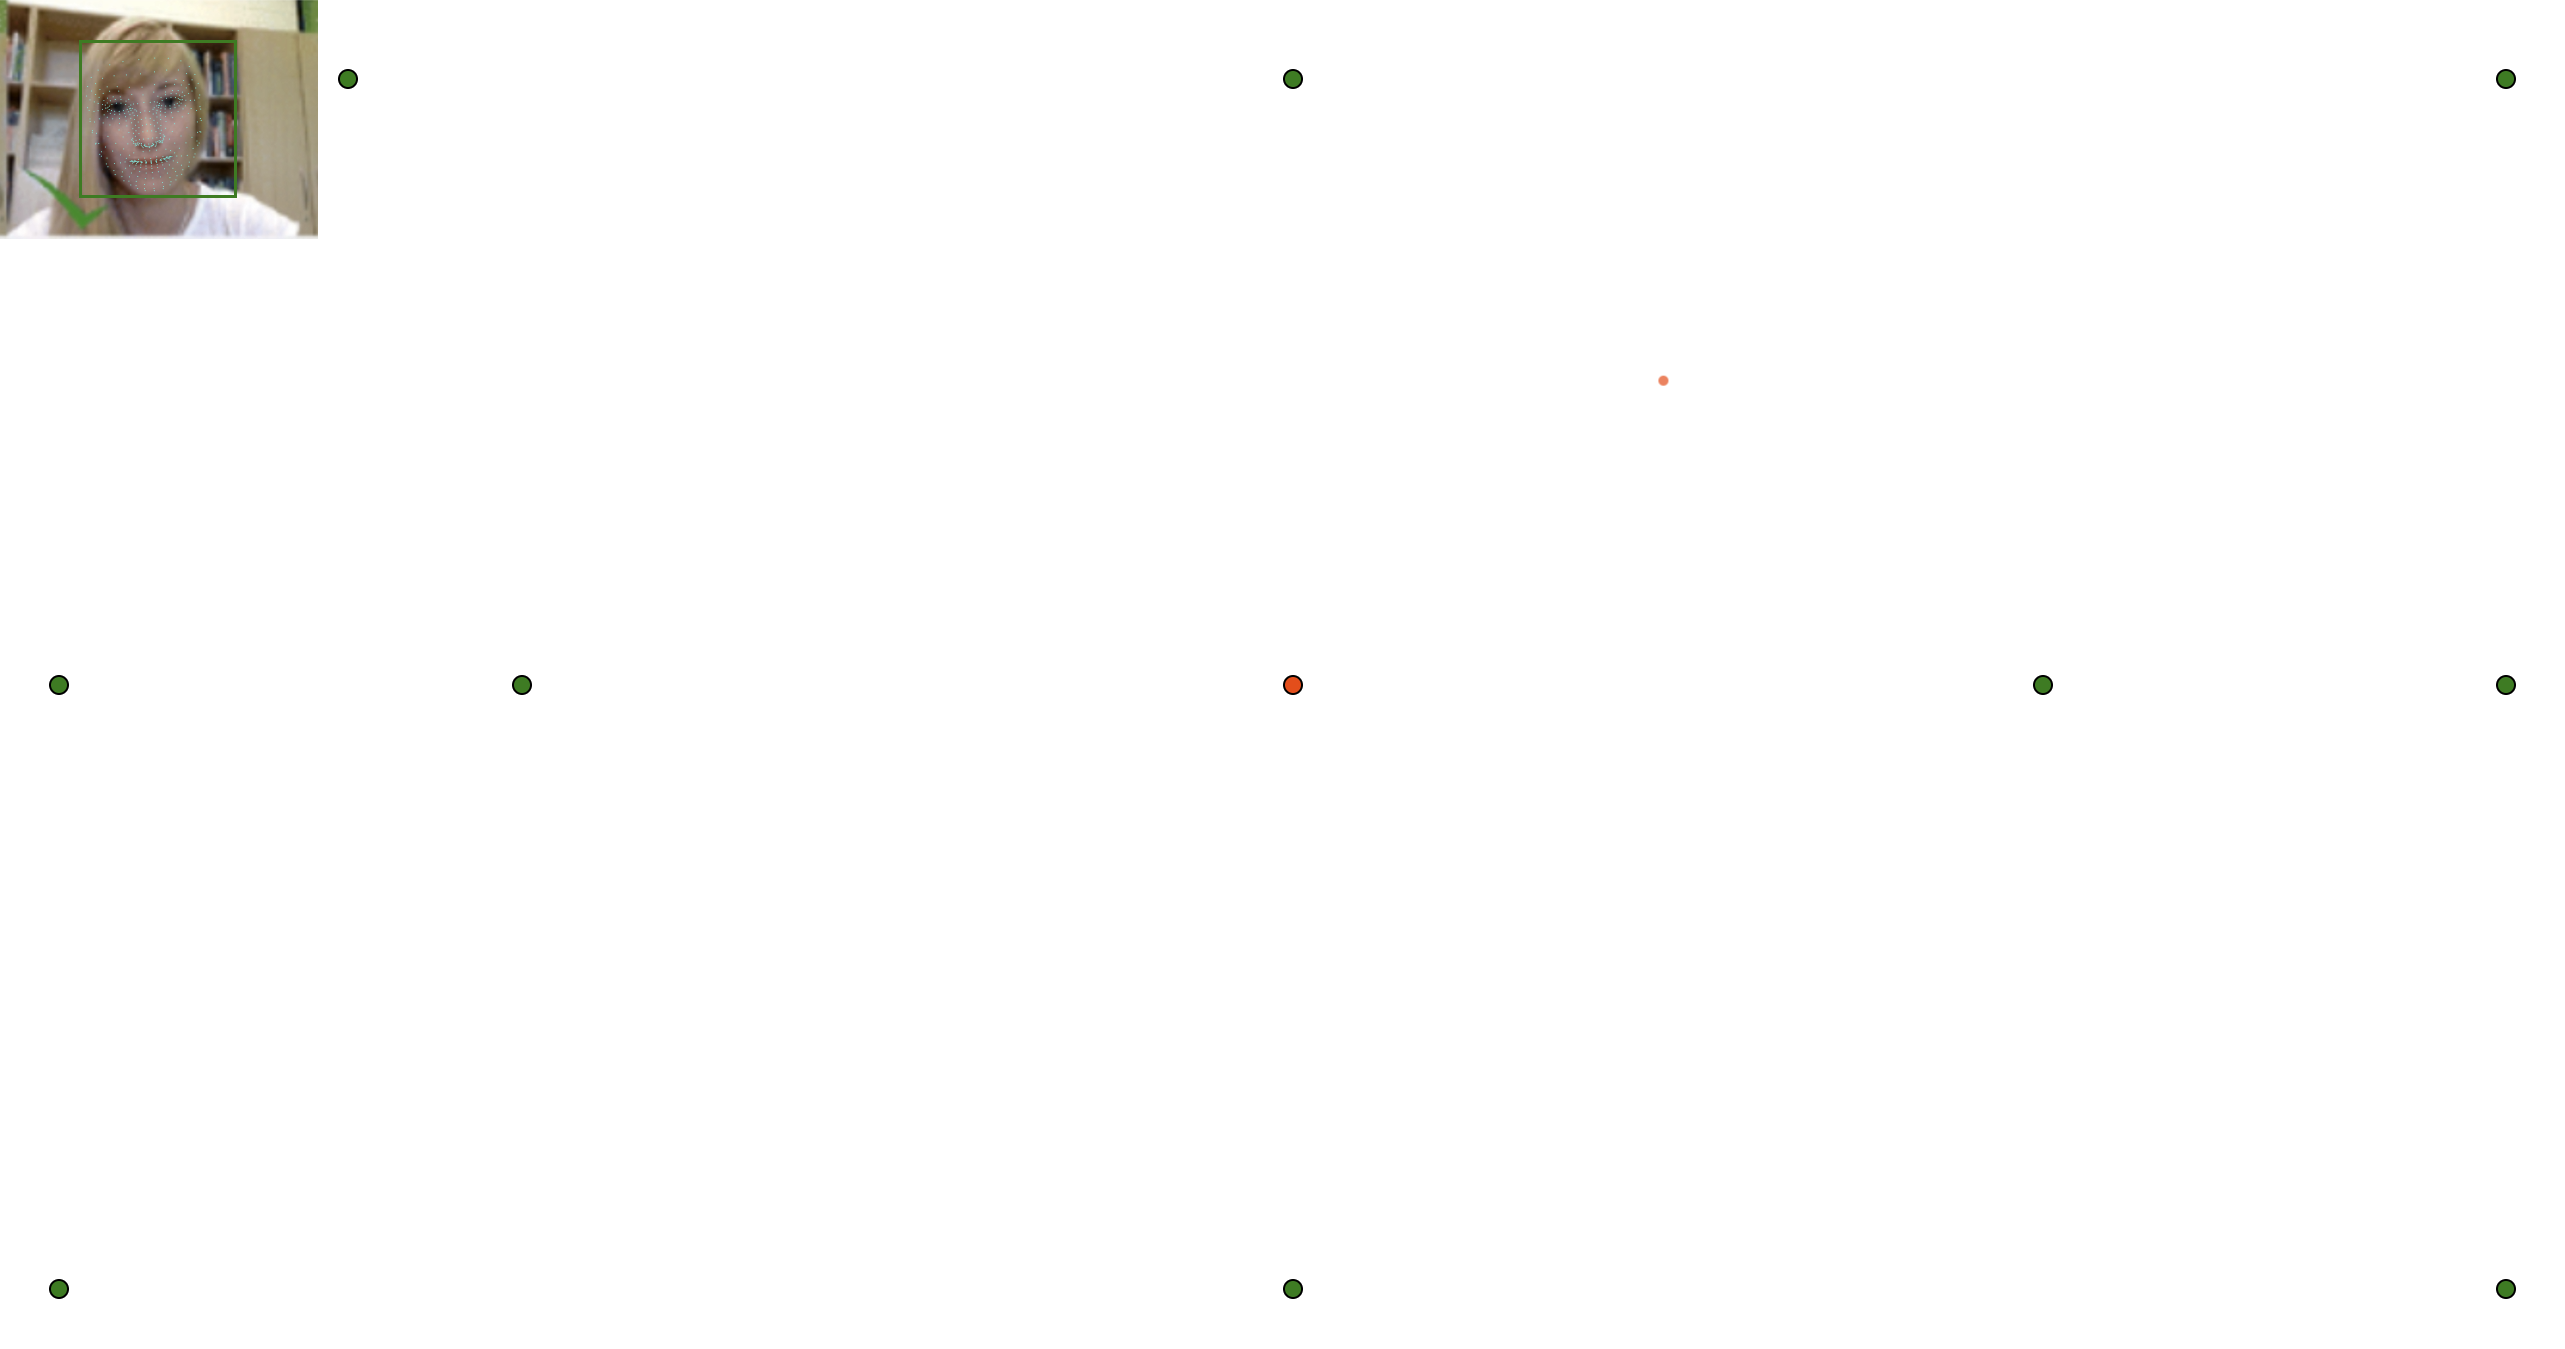
\includegraphics[width=0.8\textwidth]{images/calibration_webcam.png}}
    \caption{Calibration setup}
    \label{fig:calibration_webcam}
\end{figure}

In order to successfully pass the calibration assessment, the participants must reach at least 65\% accuracy on each of the three calibration points. However, during the testing phase we noticed that the calibration assessment was too strict and difficult to pass. Therefore, it was determined that the left and right points should be made easier to calibrate via adjusting the calculation of the accuracy. A weighted accuracy calibration procedure was implemented. While the distance for the accuracy of the middle point was calculated via euclidean distance, the left and right points were calculated via the following formula: $\sqrt{(w_x\cdot(calib\_point\_x - gaze\_x))^2 + (w_y\cdot(calib\_point\_y - gaze\_y))^2}$. Where $w_x$ and $w_y$ are the coefficients that were adjusted during the testing phase. The final values were $w_x = 1$ and $w_y = 0.5$. The values were chosen based on the fact that left and right objects do not have any other objects on the vertical axes this can be seen in \autoref{fig:example_trial_webcam}. Therefore a slightly inaccurate result on the vertical axes would be relatively easy to correct during the analysis.

The images were located on the screen as far as possible to reduce the errors as much as possible. For the same reason, the available messages were kept as a single block instead of being spread further apart. 

Furthermore, a performance issue arised during the pilot phase. The issues was that the eye tracking became very slow and laggy towards the the second half of the experiment. The more clicks were made, the worse the performance became. Due to a drastic drop in sampling rate and increase in response time, the pilot data was clearly unacceptable. The issue was resolved by reducing the \text{DataWindow} size from 700 to 50 in source code and recreating the WebGazer source file afterwards. The issue was resolved and the performance was stable throughout the experiment. 

\begin{figure}
    \centering
    \fbox{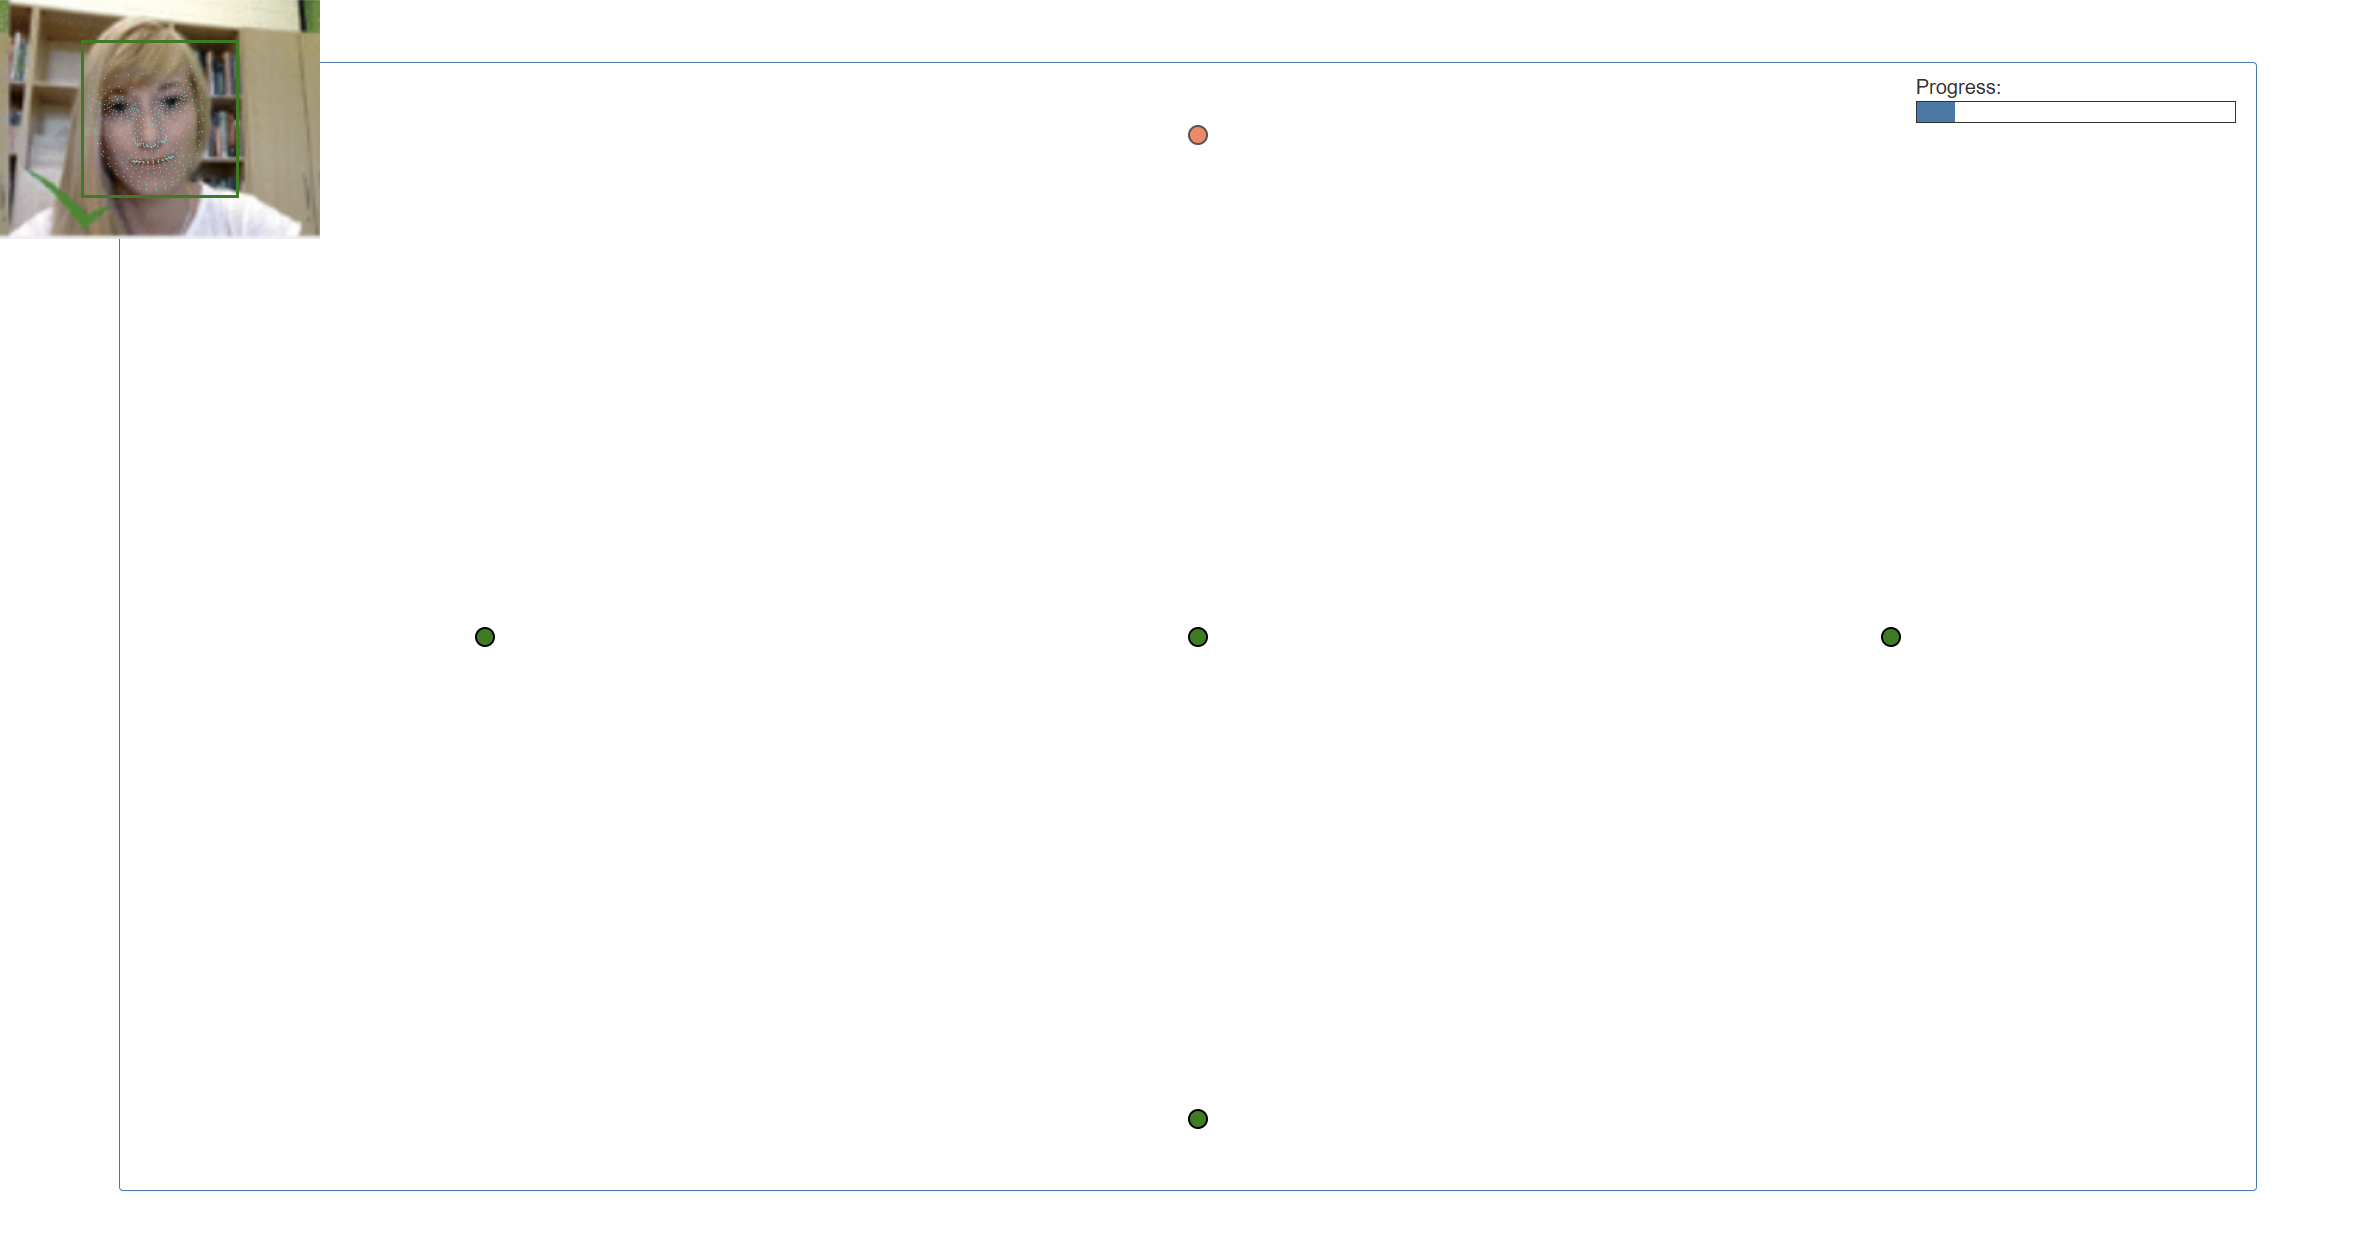
\includegraphics[width=0.8\textwidth]{images/inbetween_calibration_webcam.png}}
    \caption{In-between trial calibration}
    \label{fig:inbetween_calibration_webcam}
\end{figure}

\begin{figure}
    \centering
    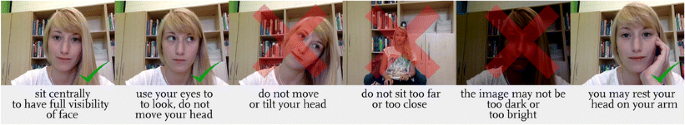
\includegraphics[width=0.8\textwidth]{images/calibration_instr.png}
    \caption{Calibration instructions taken from \cite{Semmelmann_2018}}
    \label{fig:calibration_instr}
\end{figure}

The calibration is highly dependent on the setup. Hence, the following pieces of advice were given to the participants to increase chances of successful calibration: keep the laptop on charging during the whole experiment (to make sure the eye tracking does not suffer from battery saving features); choose a quiet, well-lit room with minimal distractions and use a stable chair; place your laptop on a stable surface, screen directly in front of you. Later during the calibration, ensure the webcam is centered with your face; keep your head as still as possible during the experiment; make this window full screen size if not already. In addition, right before the calibration the participants were shown their webcam feed to make sure they are centered and the lighting is good as well as some visual advice on how to improve the calibration. The visuals can be seen in \autoref{fig:calibration_instr}. They were taken from a different experiment \citep{Semmelmann_2018} that was conducted with use of WebGazer \citep{webgazer}.

Even with all the optimizations in place, the calibration procedure was still relatively difficult to pass. The participants were not restricted in number of attempts to calibrate. However, the participants were informed that the approval is only possible after successfully completing the calibration and the rest of the experiment.

\subsection{Consent}
The participants were informed about the eye-tracking procedure at the beginning of the experiment. They were informed that no video of them will be stored at any point of time. The participants were informed that they can stop the experiment at any point by exiting the website and none of their data will be saved. The project and the consent formulation was approved by the Ethical Review Board of the Faculty of Mathematics and Computer Science at Saarland University. The exact formulation was: 

\begin{quote}
    This experiment is being conducted as part of ongoing research at Saarland University. If you have any questions or comments about the study, please contact us. You must be at least 18 years old to participate. Your participation in this research is voluntary. There are no risks or benefits to participating in this study. You may decline to answer any or all of the following questions. You may decline further participation, at any time, without adverse consequences. Part of the data collections involves using your webcam to estimate your eye gaze. No video or audio is stored at any point during the experiment. We only use the video to store the estimated position of your eye gaze, as well as estimated size of your pupil. All data will be anonymized prior to analysis. 

    If you agree to participate, please read the below instructions before proceeding.
\end{quote}


\section{Analysis}
\label{sec:analysis}

\subsection{Features}
\label{sec:analysis:features}
Considering the related eye-tracking study conducted by \cite{Vigneau_2006}, the analysis will be around the defined eye-tracking features. \cite{Vigneau_2006} defined mainly 5 types of features: absolute time on an area of interest, proportional time on an area of interest, toggling (between the Raven's matrix and the available messages), item latency (time to complete the trial) and latency to first toggle and matrix distribution index (how equally the attention was spread across the matrix items). In this study on the other hand, we are mainly focused on the proportional time on the areas of interest. The decision was made for multiple reasons. First of all the sampling rate of WebGazer is highly dependent on the participants' computer, making the absolute time on the areas of interest and latency to first fixation not comparable between participants. Second of all, we do not have such a strong hypothesis about what exactly people do during the task solving process as \cite{Vigneau_2006} had. We are rather interested in the general profile of attention, hence, no toggling features were included in the analysis. 

In addition to the eye-tracking features, we included some general features about the trial. The features are: trial number, condition (Simple, Complex or Unambiguous), type of sent message feature (shape or color), correct (whether the trial was solved correctly or not) and Target position (left, center or right). The condition and correct features play crucial role in the analysis. While the other features such as trial number, type of sent message and Target position were included due to the fact that they were shown to sometimes have a significant effect on the participants' performance in the previous studies \citep{Mayn_2023, Mayn_2025}.

\subsection{Data Preprocessing}
\label{sec:analysis:preprocessing}
The data preprocessing was done in Python using the pandas library \citep{pandas}. Firstly, due to how LingoTurk \citep{lingoturk} is implemented, we had to parse the data from string into the dictionary and create a data frame from it. As was mentioned before, the WebGazer \citep{webgazer} library was used to track the eye gaze. The WebGazer predicts the x and y coordinates of the current gaze point on the screen. Hence, we had to define a certain boundaries for the areas of interest in order to assign the predicted gaze points to them. Taking into account the weighted calibration described in \autoref{sec:data:eyetr}, which was implemented for the left and right objects we had to make the margin a little larger for the left and right objects comparing to the center one. We settled on defining four point polygons for each of the interest areas. 

The polygons were defined using the following variables: 
\begin{itemize}
    \item $x_{12}$ -- x coordinate equally distant between the left and the center images of the objects.
    \item $x_{23}$ -- x coordinate equally distant between the center and the right images of the objects.
    \item $y_{12}$ -- y coordinate equally distant between the sent message image and the center object image.
    \item $y_{23}$ -- y coordinate equally distant between the center object image and the available messages images.
\end{itemize}
It is worth to note that the values of the variables can be easily computed using the coordinates of left top corner of an image and its width and height which were saved during the experiment. Finally, the polygons were defined via four points as follows:
\begin{itemize}
    \item sent message -- $((x_{23}+\frac{x_{12}}{2}, 0), (\frac{x_{12}}{2}, 0), (x_{12}, y_{12}), (x_{23}, y_{12}))$
    \item left object  -- $((0, \frac{y_{12}}{2}), (x_{12}, y_{12}), (x_{12}, y_{23}), (0, y_{23}+\frac{y_{12}}{2}))$
    \item center object -- $((x_{12}, y_{12}), (x_{23}, y_{12}), (x_{23}, y_{23}), (x_{12}, y_{23}))$
    \item right object -- $((x_{23}, y_{12}), (x_{12}+x_{23}, \frac{y_{12}}{2}), (x_{12}+x_{23}, y_{23}+\frac{y_{12}}{2}), (x_{23}, y_{23}))$
    \item available messages -- $((x_{12}, y_{23}), (x_{23}, y_{23}), (x_{23}+\frac{x_{12}}{2}, y_{12}+y_{23}), (\frac{x_{12}}{2}, y_{12}+y_{23}))$
\end{itemize}
\begin{figure}
    \centering
    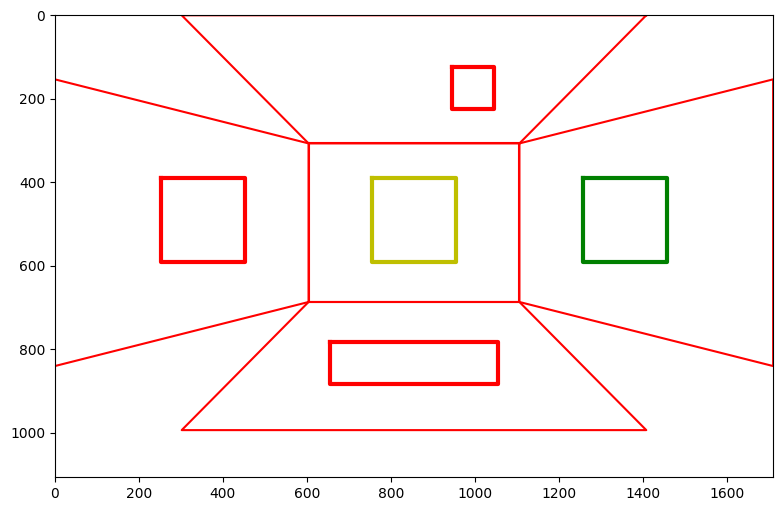
\includegraphics[width=0.8\textwidth]{images/polygons.png}
    \caption{Polygons for the areas of interest. The inner rectangles show the exact positions of the images on the participant's screen. The outer rectangles show the polygons used to define the areas of interest.}
    \label{fig:polygons}
\end{figure}
The visualization is shown in \autoref{fig:polygons}. 

\begin{figure}
    \begin{subfigure}{1\textwidth}
        \centering
        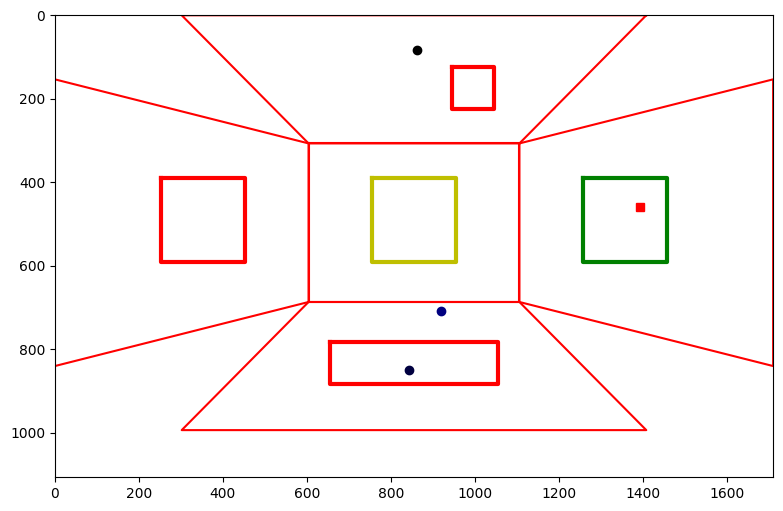
\includegraphics[width=0.7\textwidth]{images/fixations.png}
        \caption{Fixations}
        \label{fig:fixations}
    \end{subfigure}
    \begin{subfigure}{1\textwidth}
        \centering
        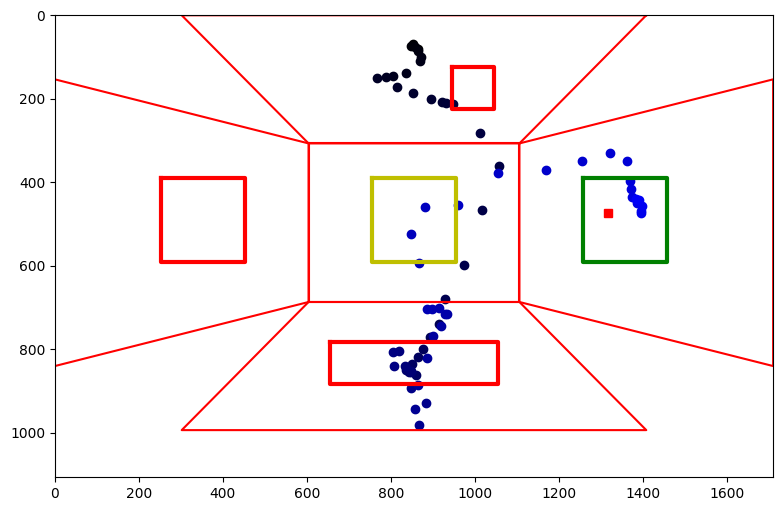
\includegraphics[width=0.7\textwidth]{images/scanpath.png}
        \caption{Scanpath}
        \label{fig:scanpath}
    \end{subfigure}
    \caption{Comparison of the raw scanpath (b) and the detected fixations (a). The hue of the points corresponds to the order of the points. Black being the first point and the pure point being the last. In addition, the very last point is marked with a red square.}
    \label{fig:fixations_scanpath}
\end{figure}

\subsection{Eye Tracking Features}
\label{sec:analysis:eyetr}
Based on whether a point was inside a certain polygon or none of them it was assigned to the corresponding area of interest or to the non-area-of-interest category. Each point was not represented by the time between the current and the previous point as the rate of sampling was not the same across participants. In order to mitigate this issue a fixation detection algorithm was tried out. The algorithm is implemented in R \citep{fixation_detection}. The algorithm is based on the fact that due to a fixation present some points would be close to each other while the rest would be far away. The algorithm states to work well even for a low quality data with sampling rate less than 100 Hz. However, in our case an average sampling rate amounted to 18 Hz. Even with the lowest tolerance, the algorithm was not able to detect all fixations accurately due to the low sampling rate. An example of fixation detection and the original scanpath can be seen in \autoref{fig:fixations_scanpath}. Here, the algorithm correctly detected 4 fixations, they are: on the sent message, twice on the bank of available messages and the last one being on the right object. While the second fixations of the available messages is debatable, clearly the algorithm was not able to detect the quick glance on the middle object before the last fixation on the right object. Clearly, the sampling rate was too low in order to determine the fixations accurately. Hence, the algorithm was not used in the analysis. 

\begin{figure}
    \centering
    \begin{floatrow}
    \ffigbox{%
      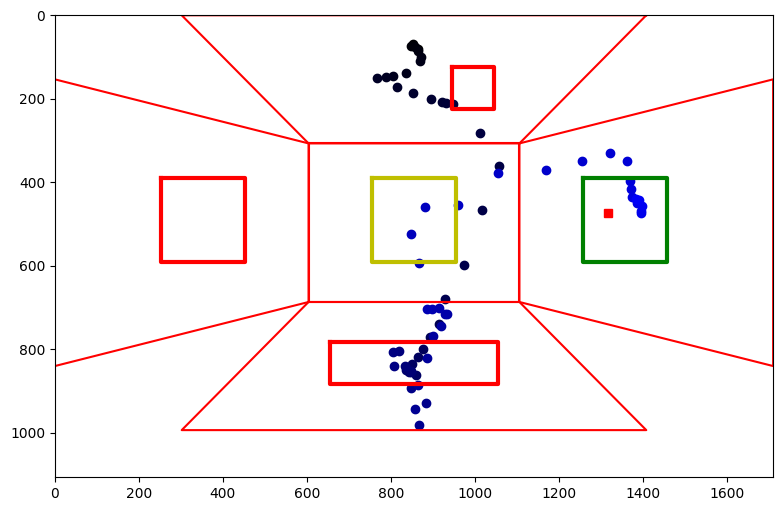
\includegraphics[width=0.48\textwidth]{images/scanpath.png}
    }{%
      \caption{Scanpath of a Simple trial, and the layout of areas of interest. The colors of the main objects are used as follows: green -- Target, yellow -- Competitor and red -- Distractor.}%
      \label{fig:features_scanpath}
    }
    \capbtabbox{%
    \begin{tabular}{|l|c|}
    \hline
    Feature & Value \\ \hline
    TimeOnSentMsg & 18 \\ 
    TimeOnAvailableMsgs & 27 \\ 
    TimeOnTrgt & 14 \\ 
    TimeOnDist & 0 \\ 
    TimeOnComp & 9 \\ 
    TimeOnNonAOI & 0 \\ 
    PropTimeOnSentMsg & 0.26 \\ 
    PropTimeOnAvailableMsgs & 0.4 \\ 
    PropTimeOnTrgt & 0.21 \\ 
    PropTimeOnDist & 0.0 \\ 
    PropTimeOnComp & 0.13 \\ 
    PropTimeOnNonAOI & 0.0 \\ \hline
    \end{tabular}
    }{%
      \caption{Features and their corresponding values. The features starting from ``Time'' corresponds to amount of points in the area of interest.}%
      \label{tab:features}
    }
    \end{floatrow}
\end{figure}

Instead of using the algorithm, we decided to use the raw scanpath and derive the features from it. We assign each predicted gaze point to the corresponding area of interest. Then count the amount of them in each area of interest. This way we derive absolute time on area of interest. Again, it is worth mentioning that we did not use the actual timings of the predictions because the sampling rate varied a lot across the participants. Hence, we used the amount of points in each area of interest as a proxy for the time spent on it. Furthermore, we calculated the proportional time on area of interest as the amount of points in the area of interest divided by the total amount of points in the trial, including the ones that missed the areas of interest. The proportional time on area of interest is the main feature used in this thesis. An example of calculated features for the scanpath in \autoref{fig:features_scanpath} can be seen in \autoref{tab:features}.



\subsection{Pairwise Correlations}
\label{sec:analysis:corr}
Similarly to \cite{Vigneau_2006}, we will report the pairwise correlations of eye-tracking features and the accuracy based on condition. This should give us some general idea about what features are correlated with the accuracy. In addition, the correlation will test some of our hypothesis.

\subsection{Mixed Effects Logistic Regressions}
\label{sec:analysis:mixed_effects}

Throughout our modeling, we assume that the data are independent and identically distributed (i.i.d.), meaning that each trial is treated as an observation drawn from the same distribution and independent of other trials. The main analysis will be done using mixed effects logistic regressions. The models are designed to correspond to our hypothesis presented in \autoref{sec:research_questions}. For the hypothesis 1 and 2, the following model was preregistered \citep{preregistration}:
\begin{verbatim}
    Correct ~ Condition + TrgtPos + Trial + 
    PropTimeOnTrgt + PropTimeOnComp + PropTimeOnDist + 
    PropTimeOnSentMsg + PropTimeOnAvailableMsgs + 
    PropTimeOnNonAOI + MsgType +
    (1 + Condition + TrgtPos + Trial + PropTimeOnTrgt + 
    PropTimeOnComp + PropTimeOnDist + PropTimeOnSentMsg + 
    PropTimeOnAvailableMsgs + MsgType | Subject)
\end{verbatim}

However, we quickly realized that the model has a few issues. First of all, the model is missing interaction between the different conditions and the eye-tracking features. Therefore, the interaction terms were added to the model. The second issue is that the feature ``PropTimeOnNonAOI'' can be derived from the other eye-tracking features making it redundant and unnecessary to include in the model, hence, it was removed. In addition, we added the ``AnswerTime'' feature to the model. The ``AnswerTime'' feature is the time between the start of the trial and the moment when the participant clicked on the answer. It was added to account for the fact that some participants might have been faster than others. The final starting model looks as follows:

\begin{verbatim}
    Correct ~ Condition + TrgtPos + Trial + 
    PropTimeOnTrgt + PropTimeOnComp + PropTimeOnDist + 
    PropTimeOnSentMsg + PropTimeOnAvailableMsgs + MsgType +
    AnswerTime +
    Condition:PropTimeOnTrgt + Condition:PropTimeOnComp +
    Condition:PropTimeOnDist + Condition:PropTimeOnSentMsg +
    Condition:PropTimeOnAvailableMsgs + Condition:AnswerTime +
    (1 + Condition + TrgtPos + Trial + PropTimeOnTrgt + 
    PropTimeOnComp + PropTimeOnDist + PropTimeOnSentMsg + 
    PropTimeOnAvailableMsgs + MsgType + AnswerTime | Subject)
\end{verbatim}

Through this model we will be able to test the first two hypothesis. Mainly whether the Distractor is positively associated with the accuracy on the Complex trials. And, for the second hypothesis, whether the available messages become important on the Simple trial comparing to Unambiguous and maybe Complex as well. The model will be fit on the trial level and predicts whether the answer was correct or not. The ``Trial'' and ``AnswerTime'' features were rescaled to be between -1 and 1, in order to match the scale of other features. All the eye-tracking features were centered to have mean 0 but not scaled. This approach was chosen because it would make the interpretability of the models easier.

As for the third and fourth hypothesis, each of them will be tested using a separate model. These models treat each fixation as an independent observation. Accordingly, we assume the gaze data to be i.i.d., meaning that each fixation is considered to be drawn independently from the same probability distribution. Both of them predict whether a gaze point was on a certain area of interest. Hence, the data to fit them is made on the gaze point level. Only the gaze points from the correctly solved trials were added to the data to match the hypothesis. The third hypothesis will be tested using the following model:
\begin{verbatim}
    OnDist ~ Condition + Trial + MsgType + TrgtPos +
    (1 + Condition + Trial + MsgType + TrgtPos | Subject)
\end{verbatim}
It predicts whether a gaze point was on the Distractor or not based on the general information about the trial. 

The fourth hypothesis will be tested using the following model:
\begin{verbatim}
    OnAvMsgs ~ Condition + Trial + MsgType + TrgtPos +
    (1 + Condition + Trial + MsgType + TrgtPos | Subject)
\end{verbatim}
It predicts whether a gaze point was on the bank of available messages or not based on the general information about the trial. 

